\chapter{Schlusswort}
\color{blue}
Der \textsc{Detroit Electric Car} zeigt sehr gut, dass sich in den letzten einhundert Jahren im grundsätzlichen Bereich der Elektromobilität nicht viel verändert hat: So wird bereits im Oldtimer der Motor über die Spannung und das Feld geregelt. Das heute dazu oftmals ein anderer Motorentyp verwendet wird, sei einmal ausser Acht gelassen. In der Schaltung des \textsc{Detroits}, welche als genial bezeichnet werden muss, wird lediglich beim Anfahren zur ersten Fahrstufe Wärme in einem Widerstand umgesetzt.

Grosse Umbauten am Fahrzeug wurden nicht umgesetzt, um möglichst vieles im Originalzustand zu belassen. An einigen Stellen war dies jedoch unausweichlich, um so die Funktion und Sicherheit zu gewährleisten. Ebenfalls modifiziert wurden Baugruppen, welche nicht mehr dem Originalzustand entsprachen und somit keinen historischen Wert aufwiesen.

Die zu verwendende Batterie, welche aus einem verunfallten modernen Elektrofahrzeug stammt, konnte auf das Fahrzeug abgestimmt werden. Trotzdem wurden dabei nicht die modernen Funktionen, welche zur Funktions- und Sicherheitsüberwachung von Lithium-Ionen-Zellen nötig sind, vernachlässigt. Für das Fahrzeug resultiert aber, abgesehen vom deutlich kleineren Innenwiderstand der neuen Batterie, kein Unterschied in der Funktionsweise.

Die Arbeiten am \textsc{Detroit} konnten abgeschlossen werden. Auf Probefahrten hat sich gezeigt, \textcolor{red}{dass sämtliche Funktionen korrekt funktionieren}. Trotzdem wurden dabei wichtige Erkenntnisse gewonnen. Am wichtigsten sei hier sicherlich die Reichweite zu nennen. Hier lagen erste Schätzungen deutlich daneben, beträgt die Reichweite bei realistischer Fahrweise doch nur ungefähr 100 km.

\begin{figure}[h]
	\centering
		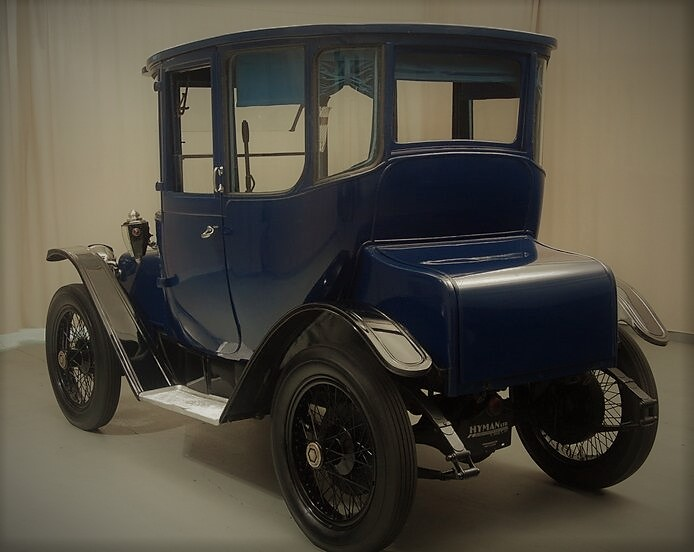
\includegraphics[width=0.75\textwidth]{images/Ende.jpg}
	\label{fig:Ende}
\end{figure}


\color{black}